\chapter{\TitreChapitreQuatre}\label{chap:Convoyeur}

\bfigh
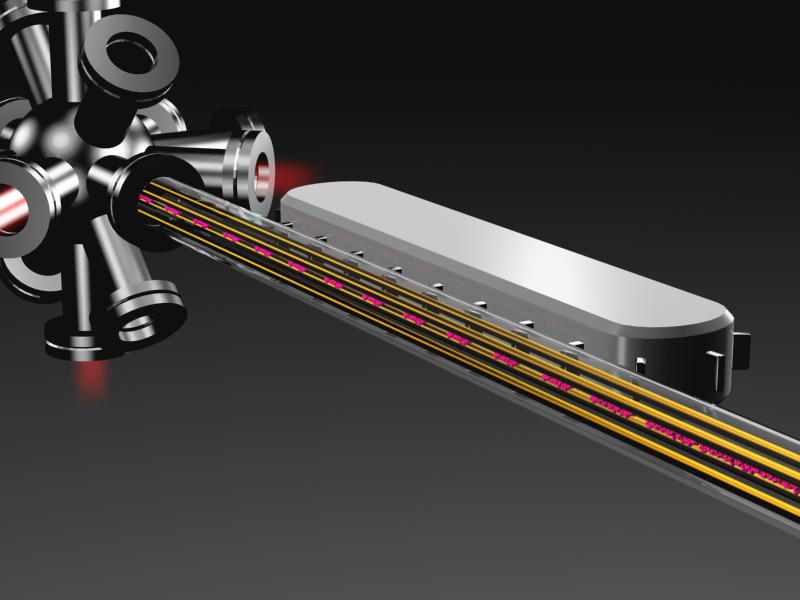
\includegraphics[width=\FigWidth]{P2/ChapitreConvoyeur}
\SansCaption
\efigh

\pagebreak
\Cahier{Début de l'étude : 7,164}

\minitoc
\vspace{0.5cm}

\section{Transport de \patufs : introduction}\label{sec:ConvIntro}

\subsection{Enjeu général}
Le transport de \patufs a connu un développement remarquable ces dernières années. La motivation initiale résidait dans le transport d'une chambre de préparation de ces nuages d'atomes vers une autre chambre où le vide, de bien meilleure qualité, était mis à profit pour étudier le régime de dégénérescence quantique dans des conditions optimales.

Les premières expériences combinant deux chambres à vide utilisaient alors deux \pmos. Le premier assurait le chargement et le refroidissement d'un nuage d'atomes qui, lancé ou tombant simplement sous l'effet de la gravité, était récupéré dans une autre chambre par le deuxième piège~\cite{CMW91}. Dans d'autres dispositifs, le deuxième piège est alimenté par un jet d'atomes froids, réalisé grâce à un \pmo comportant un axe de fuite~\cite{LCR96, DSW98}. 

Une nouvelle génération de \setups a ensuite vu le jour avec la mise en place d'un seul \pmo et d'un système de transport magnétique ou optique des atomes froids vers la seconde chambre à vide. Cette dernière permet de bénéficier d'un accès optique optimal. 

\casse

\inlinefig{\begin{minipage}{6.6cm}
\vspace{1pt}\hspace{1pt} 
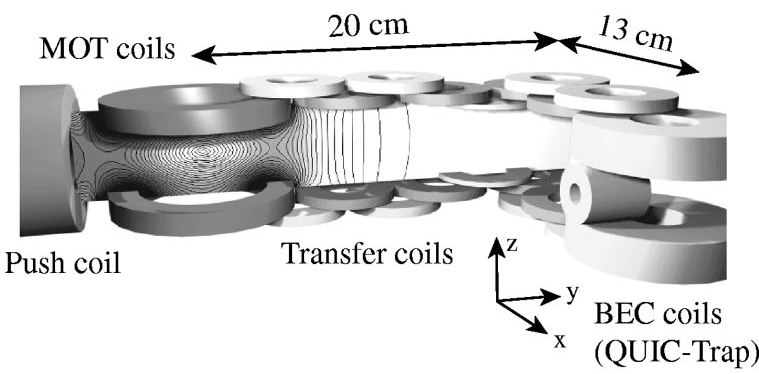
\includegraphics[width=6.4cm]{P2/TransportHansch}~\\
\RemonteUnPeuFig \RemonteUnPeuFig \RemonteUnPeuFig \RemonteUnPeuFig \RemonteUnPeuFig 
\begin{center}{Image issue de la référence~\cite{GBH01}}\vspace{2pt}\end{center}%%
\end{minipage}}
L'équipe du professeur Theodor Hänsch de l'université de Munich a développé dès 2001 un transport magnétique sur une distance de \cm{30}~\cite{GBH01}. Le principe de sa méthode repose sur l'utilisation d'un enchevêtrement de paires de bobines dans lesquelles des courants alternés permettent de déplacer le minimum d'un potentiel magnétique (voir l'illustration ci-contre). 
\picskip{0}
\noindent Ce même groupe propose la même année une version miniaturisée d'un dispositif de transport magnétique en imprimant, par lithographie sur une \termetech{puce à atomes}, les fils conducteurs qui génèrent les \chms~\cite{HRH01}. Ce type d'approche permet même de transporter des \bec~\cite{HHS05}. 
L'équipe d'Eric Cornell de l'université de \nomofficiel{Boulder} (USA) utilise depuis 2002 un système de transport magnétique qui consiste à déplacer mécaniquement une paire de bobines~\cite{LHW03, NSH05}. 

Le transport d'atomes froids s'effectue également par des moyens purement optiques. Le groupe du professeur Wolfgang Ketterle (\nomofficiel{Massachusetts Institute of Technology}) a ainsi mis au point en 2002 une \termetech{pince optique} autorisant le transport sur plus de \cm{40} d'un \bec~\cite{GCL02}. Une autre méthode optique de transport consiste à produire un réseau de pièges optiques en mouvement en utilisant les interférences entre deux faisceaux lasers contrapropageants~\cite{STW06,MGW03}.
%Nous discuterons plus en détails des expériences de transport de \natufs dans le chapitre \vref{chap:PiegeDipolaire}. 
Ces innovations ont depuis largement été reprises et adaptées par un grand nombre de groupes de recherche travaillant sur des gaz quantiques dégénérés. 


\subsection{Logique de cette approche pour la formation d'un \jatuf}

La motivation de notre équipe vis-à-vis du transport de \patufs diffère sensiblement du cadre dans lequel ces premières études ont été menées. Nous souhaitions en effet mettre au point le transport, non pas d'un seul \p, mais de \emph{plusieurs \ps simultanément} sur une partie du \gm. Nous expliquons ci-dessous l'intérêt de mettre au point un tel \setup.
%\cite{}.
%Ceux-ci sont destinés à traverser des zones d'évaporation au fil de leur avancée, puis à être relâchés dans le \gm. 


\subsubsection{Rappel : les trois difficultés inhérentes à l'évaporation d'un \jatg}
\`A la fin du chapitre~\nref{chap:JetAtomique}, nous avons mentionné trois raisons expliquant pourquoi l'\evap d'un \jat est une tâche fondamentalement plus ardue que celle d'un nuage piégé. Rappelons brièvement ces trois points :
\begin{itemize}
	\item l'injection pulsée implique une \emph{dilution spatiale} des \ps suivant l'axe du \gm. Ceci se traduit par une perte en \dat, et donc en \tcolel.
	\item le guide ayant une longueur finie, le temps alloué pour réaliser l'évaporation est limité par la vitesse moyenne du jet. En pratique nous disposons d'environ \seconde{6}.
	\item le \emph{confinement purement transverse} rend le processus d'évaporation moins efficace que dans le cas d'un piégeage suivant les trois dimensions. Il est en particulier impossible d'observer un emballement de l'évaporation dans un \ppthar%
\footnote{Les lois d'échelle pour l'évaporation à 2 dimensions sont en effet nettement moins favorables qu'avec un piégeage \td~\cite{LaG06,DMK95,KeV96}.}. 
\end{itemize}
Nous avons donc conclu à la nécessité de développer de nouveaux outils visant à améliorer les conditions d'évaporation dans le \gm. Ainsi, dans le chapitre~\nref{chap:MiroirMobile}, nous avons décrit une technique permettant de ralentir les \pats par réflexion sur un \mimamo. Le jet ainsi formé par recouvrement de ces \ps est plus lent et plus dense. Ceci répond donc a priori aux deux premières difficultés citées ci-dessus.



\subsubsection{Pour aller plus loin}

La mise en \oe uvre de la technique du \mimamo est instructive puisqu'elle nous a permis de mettre en évidence les possibilités liées à l'utilisation d'un potentiel dépendant du temps afin d'agir sur les degrés de liberté externes des atomes.

Dans ce chapitre, nous allons présenter une technique originale permettant de maintenir momentanément un piégeage \td dans le \gm. Pour ce faire, les \ps successivement injectés dans le guide sont immédiatement recapturés dans un \tpm en mouvement. 

Nous commencerons ce chapitre par l'étude des caractéristiques du confinement dans le \tp. Nous étudierons ensuite les paramètres intervenant lors du piégeage et du transport d'un \pat. Nous expliciterons, avec l'appui de simulations numériques, les mécanismes physiques à l'\oe uvre dans ce problème de transport multiple. 
%Nous détaillerons ons les limites de notre premier dispositif, et les perspectives ouvertes par nos travaux. 
Nous présenterons enfin les résultats démontrant le transport ainsi que le refroidissement des paquets piégés dans le \tpm.


\section{Un train de pièges magnétiques à aimants permanents}\label{sec:ConvTrainAimants}

Cette section a pour but de détailler le \setup permettant de produire un \tp ainsi que les caractéristiques du confinement magnétique correspondant. 
\Remarque{
Rappelons que le confinement transversal des atomes est assuré par le guide qui fournit un \gtchm $\gradB$ (voir la \autoref{sec:ConfigMagnetiqueGuide}). Dans tout ce chapitre, il sera question d'une valeur de $\gradB = \gausspcm{800}$. 
}
Le principe de piégeage suivant la dimension longitudinale de l'axe $z$ du guide est directement inspiré de la technique du \mima. La modulation du \chm longitudinal $\Bpara(z)$ induit une variation de l'énergie potentielle le long de l'axe $z$. 



Afin de créer un \tp, nous avons mis en place des aimants permanents%
%
\footnote{Ce sont les mêmes aimants permanents que nous avons utilisés pour l'évaporation sur une pièce de céramique (\autoref{sec:EvapCeramAimants}), et pour la mise en \oe uvre du \mimamo (\autoref{sec:MiroirMiseEnMouvement}). Leurs caractéristiques principales sont données dans l'Annexe \ref{annexe:ModelisationAimants}.}
%
sur la \couconv dont les caractéristiques ont déjà été détaillées dans la \autoref{sec:MiroirMiseEnMouvement} traitant de la mise en mouvement du \mimamo. Cette courroie comporte $50$ sites de fixation espacés de \cm{5}. 

\casse


La figure~\nref{fig:ConvMontageAimant} montre la manière dont les aimants sont disposés:
\begin{itemize}
	\item tous les \cm{5} sur la \couconv longeant le guide,
	\item avec l'aimantation suivant l'axe $z$ du guide,
	\item les aimants de deux sites consécutifs sont dirigés dans des directions opposées.
\end{itemize}
\bfigh
\subfloat{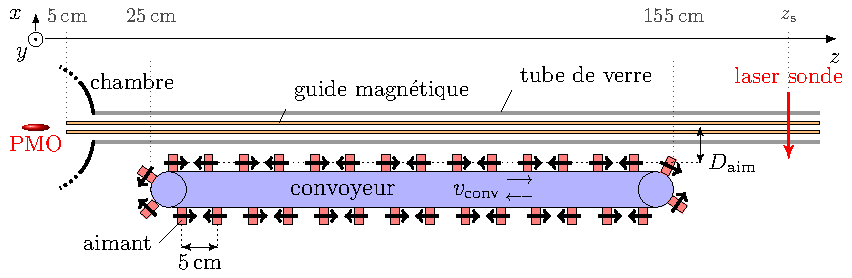
\includegraphics{P2/ConvMontageAimant}}\\
\subfloat{\includegraphics{P2/conv_photo_DSC05141}}
\CaptionFig{La \couconv longe le tube de verre du \gm sur une longueur de \cm{120}. Elle comporte $50$ sites de fixation espacés de \cm{5}. Sur chacun d'eux, un ou plusieurs aimants permanents sont fixés, l'aimantation s'exerçant selon l'axe $z$. Les aimants de deux sites consécutifs sont dirigés dans des directions opposées de manière à produire la configuration de \chm illustrée sur la figure~\nref{fig:ConvChampQP}. 
Un \pat injecté dans le guide se propage librement jusqu'en $z\approx\cm{25}$ où l'influence du champ fourni par les aimants se fait sentir.
Un \lsonde permet de mesure la \datlin $n(z=\zsonde,t)$ dans le guide (voir la \autoref{sec:MesureDensiteGuide}). 
%Notons qu'une plaque de $\mu$-métal de $\cm{40x40}$ (non représentée) sert à protéger la chambre du \pmo de l'influence des aimants du \conv.
Sur la photographie du \setup on distingue le convoyeur longeant le \gm. La chambre du \pmo se trouve dans le coin supérieur droit de l'image et les \pats se propagent vers la gauche.
}
\label{fig:ConvMontageAimant}
\efigh
Notons qu'il est possible, sur chaque site de la courroie, de fixer plusieurs aimants de manière à obtenir une modulation plus intense du \chm. En pratique, nous avons conduit des expériences, avec \val{1}, \val{2} ou \val{3} aimants sur chaque site.

\EnFaitNon{
\bfigh
%\includegraphics[width=\FigWidth]{P2/conv_photo_DSC05141}
%\movie[width=6cm,height=4cm,autostart,loop,poster]{}{videos/MOV05127_NEW.MPG}
%\includemovie[autoplay,repeat,poster,textee={\includegraphics[width=\FigWidth]{P2/conv_photo_DSC05141}}]{6cm}{4cm}{videos/MOV05127_NEW.MPG}
\CaptionFig{Photographie du \setup. On distingue le convoyeur longeant le \gm. La chambre du \pmo se trouve dans le coin supérieur droit de l'image et les \pats se propagent vers la gauche.}
\label{fig:ConvPhoto}
\efig
}

\casse

\subsection{Obtention d'un train de \pmqps}
Dans le \gm, le piégeage des atomes suivant l'axe $z$ est assuré par la modulation de la composante longitudinale $\Bpara(z)$.
La mise en place de la chaîne d'aimants le long du guide conformément à la figure~\nref{fig:ConvMontageAimant} produit une configuration de \chm dont la figure~\nref{fig:ConvChampQP} représente, dans le plan horizontal $(x,z)$, quelques lignes de champ ainsi que quelques lignes équipotentielles. 
\bfigh
\subfloat{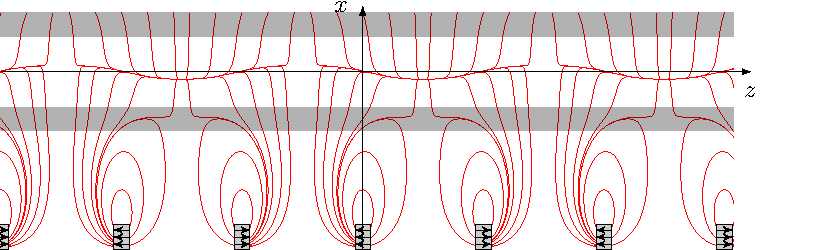
\includegraphics{P2/ConveyerChampMagnetique}}\\
\subfloat{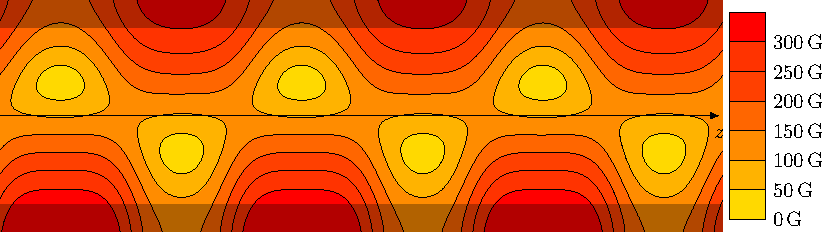
\includegraphics{P2/ConveyerEquipot}}
\CaptionFig{Allure de quelques lignes de champ et de quelques lignes équipotentielles (pour lesquelles le module du \chm est constant). En superposant le champ produit par les aimants à celui du \gm nous obtenons une succession de \pqps tridimensionnels décalés transversalement de part et d'autre de l'axe du guide. La profondeur de ces pièges est contrôlée en ajustant la distance $\ConvDaimant$ séparant les aimants de l'axe du guide.}
\label{fig:ConvChampQP}
\efigh

\noindent Le \chm produit par la chaîne d'aimants est ainsi caractérisé:% par le fait que:
\begin{itemizel}
	\item le module de $\Bpara(z) = \ConvBparaAim(z)$ %
	\nome{\ConvBparaAim}{Composante longitudinale du \chm produit par la chaîne d'aimants}%
	s'annule dans chaque plan médian%
	\footnote{En affirmant ceci, on néglige les effets de bord, \cad que l'on néglige le fait que la chaîne d'aimants n'est pas infinie.} %
	séparant deux aimants successifs (plan d'anti-symétrie pour l'aimantation),
	\item la composante transverse $\ConvBtrans$%
	\nome{\ConvBtrans}{Composante transverse du \chm produit par la chaîne d'aimants}%
	, elle, y est maximale. En ajoutant la contribution du \gtchm du guide, nous obtenons l'annulation de $\Btrans = \ConvBtrans + \Btransguide$, non plus sur l'axe $z$, mais le long d'une ligne déviée %
	\footnote{Cette ligne dévie de l'axe $z$ du fait de la modulation spatiale du \chm transverse produit par les aimants. C'est ce principe qui est mis en \oe uvre dans le chapitre~\nref{chap:Ceramique}, traitant de l'évaporation du jet en déviant sa trajectoire vers une surface matérielle.}
%
de l'axe.
\end{itemizel} 
%
\Resultat{%
La superposition du champ fourni par les aimants à celui du guide conduit donc à une succession de \pqps tridimensionnels espacés de $\ConvDqp = \cm{5}$ et répartis successivement de part et d'autre de l'axe du guide. Les pièges sont situés dans les plans médians entre deux aimants successifs. Nous produisons donc, tout au long des \cm{120} du \conv, environs $20$ \pmqps.%
}
%
La mise en mouvement de la \couconv à une vitesse constante $\vconv$ %
\nome{\vconv}{Vitesse du \tp}%
entraîne la chaîne d'aimants et permet de transporter des \pats le long du \gm. 
La figure~\nref{fig:ConvAnimQPChampLong} représente les variations de la composante longitudinale $\ConvBparaAim(z)$ du \chm produit par les aimants au voisinage de l'axe $z$ du guide.
\bfigh
\subfloat{%
\ifthenelse{\NoAnimationsInFigures > 0}{%
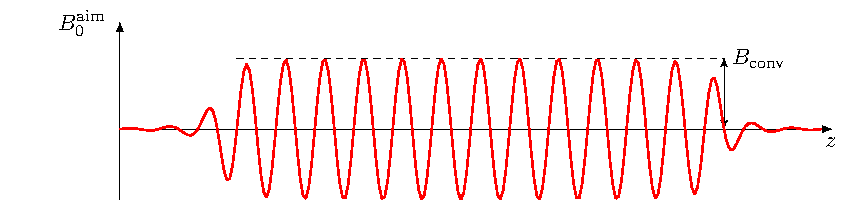
\includegraphics{P2/ConvAnimQPChampLong_1}%
}{%
\animategraphics{10}{images/P2/ConvAnimQPChampLong}{}{}}%
}\\
\subfloat{%
\ifthenelse{\NoAnimationsInFigures > 0}{%
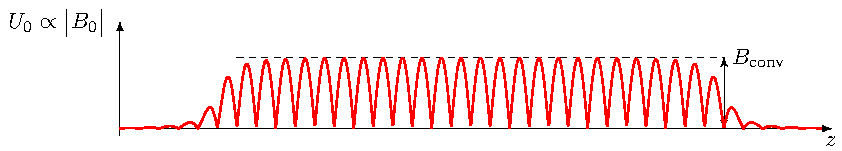
\includegraphics{P2/ConvAnimQPChampLongModule_1}%
}{%
\animategraphics{10}{images/P2/ConvAnimQPChampLongModule}{}{}}%
}
\CaptionFig{%
\AnimateOnline Allure de la composante longitudinale $\Bpara(z)$ du \chm sur l'axe $z$ du guide pour la configuration représentée sur la figure~\nref{fig:ConvMontageAimant}.
Le potentiel magnétique $\ConvUaxe(z,t)$ auquel sont soumis les atomes est proportionnel au module du champ $\left\lvert{\Bpara}\right\rvert$. 
La configuration obtenue est celle d'un \tpqpt, pour laquelle le champ s'annule ponctuellement. L'espacement entre deux pièges successifs est $\ConvDqp = \cm{5}$.%
}
\label{fig:ConvAnimQPChampLong}
\efigh


\subsubsection{Profondeur des \pqps}
La profondeur des \pqps est déterminée par l'amplitude $\ConvBamplit$ %
\nome{\ConvBamplit}{Amplitude des variations du \chm longitudinal sur l'axe du guide}%
des variations du \chm longitudinal $\Module{\ConvBparaAim(z)}$ au voisinage de l'axe du guide. Pour le \setup représenté sur la figure~\nref{fig:ConvMontageAimant}, $\ConvBamplit$ dépend de plusieurs paramètres, à savoir:
\begin{itemize}
	\item les caractéristiques des aimants permanents,
	\item la distance $\ConvDaimant$ à laquelle se trouve les aimants de l'axe du guide,
	\item le nombre d'aimants fixés sur chaque \scc.
	\item l'espacement des sites de fixation sur la \couconv.
\end{itemize}
%

\pagebreak

Pour de simples raisons d'encombrement, la distance $\ConvDaimant$ séparant les aimants de l'axe $z$ du guide est d'au moins \mm{35}. Pour une configuration avec 2 aimants par site, nous mesurons%
\footnote{L'amplitude $\ConvBamplit$ varie en fonction de la distance $\ConvDaimant$ en suivant une loi de décroissance exponentielle. Ceci est dû au caractère multipolaire de l'agencement des aimants.}
%
 :
\begin{align}
\ConvBamplit &\approx \gauss{55} \mbox{, avec }\ConvDaimant=\mm{35}\virguleformule \nonumber \\
\ConvBamplit &\approx \gauss{25} \mbox{, avec }\ConvDaimant=\mm{45}\virguleformule \nonumber \\
\ConvBamplit &\approx \gauss{9} \mbox{, avec }\ConvDaimant=\mm{55} \nonumber
\virguleformule
\end{align}
Pour $\ConvDaimant=\mm{35}$ la composante transverse du \chm produit par les aimants atteint $\Btrans \approx \gauss{40}$.

\ApplicationNumerique{
\Cahier{7,179}
Évaluons la profondeur des \pqps. 
Rappelons que nous considérons des atomes de \Rb piégés dans l'état $\EtatSFmF{1}{-1}$. Considérons une configuration à deux aimants par site, positionnés à $\ConvDaimant=\mm{35}$ de l'axe $z$. On a donc $\ConvBamplit \approx \gauss{55}$ et la profondeur des pièges est :
\[
\ConvUaxe = \mu\,\ConvBamplit = \SI{1.4E{-26}}{\joule}
\pointformule
\]
Ceci correspond à une température $T\approx\milliK{1}$ ou encore à une énergie cinétique $\tfrac{1}{2}\,m\,v^2$ avec $v = \cmps{40}$.

Du fait de la valeur élevée du champ transverse $\Btrans \approx \gauss{40}$ produit par les aimants au niveau des \pqps, ces derniers sont décalés de l'axe du guide d'une distance (voir le chapitre~\nref{chap:Ceramique}) :
\[
\Devi = \frac{\Btrans}{\gradB} \approx \mm{0,5}
\pointformule
\]
Cette valeur est à mettre en regard du rayon interne $\CeramRay = \mm{1,5}$ des \pdecs à travers lesquelles les atomes doivent passer lors de leur propagation dans le \gm. Pour une telle déviation $\Devi$, certains atomes énergétiques seront éliminés des pièges pendant le transport (voir la \autoref{sec:ResultatVariationFlux}).
}
Nous pouvons donc souligner deux défauts majeurs du piégeage dans un \tpqp:
\begin{itemize}
	\item la présence dans chaque piège d'un point de \chm nul est gênante si nous envisageons le \rpe des \pats, et ce à cause des pertes par retournement de spin.
	\item le décalage $\Devi$ des pièges hors de l'axe $z$ du guide peut conduire à l'élimination non contrôlée d'atomes du fait de la présence des \pdecs réparties sur toute la longueur du guide.
\end{itemize}
%
La \autoref{sec:ConvTrainIP} montrera comment nous pouvons contourner ces deux défauts en produisant un \tpIP.
Nous avons toutefois brièvement étudié le transport de \pats dans un \tpqp. Les résultats correspondant font l'objet de la sous-section suivante.


\casse


\subsection{Piégeage d'un \pat dans un \tpqp}
\Cahier{from : 7,166}
Dans toute la suite de ce chapitre les résultats présentés concernent des expériences faisant intervenir des paquets contenant typiquement $\val{E9}$ atomes, préparés puis injectés dans le guide suivant la procédure décrite dans la \autoref{sec:PaquetsPmo}. 

Dans cette sous-section, nous étudions l'influence du \tpqp sur la propagation d'un \pat dans le \gm. Pour ce faire, nous plaçons le \lsonde à une distance $\zsonde=\m{1,75}$, soit \cm{20} après le \conv%
\footnote{Rappelons que l'origine de l'axe $z$ est prise au niveau du \pmo.}%
. Les figures~\nref{fig:ConvSignalQP1pkt} et~\nref{fig:ConvSignalQP1pktRalenti} représentent les mesures de \datlin $n(\zsonde,t)$ obtenues dans différentes configurations:
\begin{itemize}
	\item avec une vitesse du \conv $\vconv$ égale à la vitesse d'injection $\vinj$, mais pour différentes profondeurs des \pqps, $\ConvBamplit = \gauss{0}$, $\gauss{9}$ et $\gauss{55}$ (figure~\nref{fig:ConvSignalQP1pkt}),
	\item avec une profondeur fixée, mais pour différentes vitesses du \conv, $\vconv < \vinj$ (figure~\nref{fig:ConvSignalQP1pktRalenti}).
\end{itemize} 

\bfighs
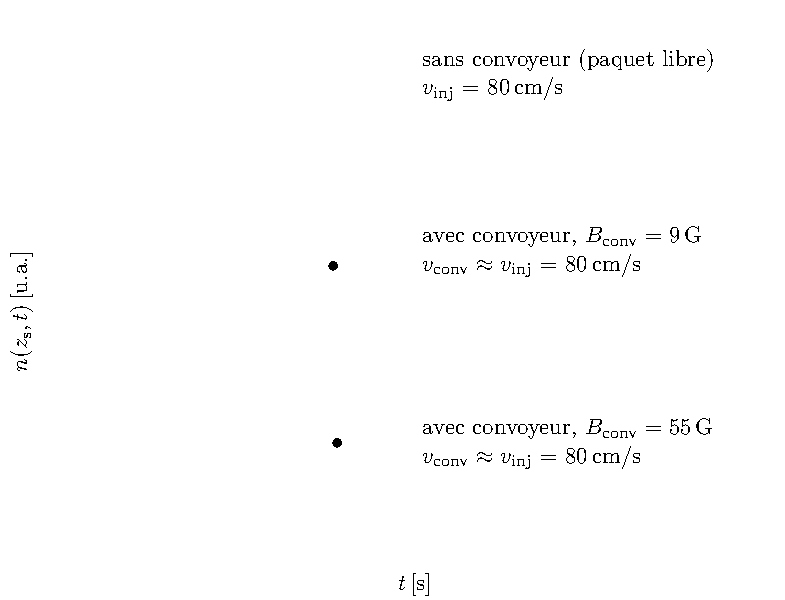
\includegraphics{P2/ConvSignalQP1pkt}
\CaptionFigs{Mesure de l'influence du \tpqp sur la propagation d'un \pat dans le \gm. Le \lsonde est positionné en $\zsonde=\m{1,75}$ (\cm{20} en aval du \conv) et mesure la \datlin $n(\zsonde,t)$ en fonction du temps $t$ après l'injection. En l'absence de \conv, le signal de détection perdure pendant plusieurs secondes, signe de l'étalement spatial durant la propagation du \p. En présence d'un \tpqp animé d'une vitesse $\vconv=\vinj=\cmps{80}$, et dont la profondeur correspond à $\ConvBamplit=\gauss{9}$, une petite partie des atomes arrive de manière groupée (pics repérés par le symbole $\bullet$). Avec $\ConvBamplit=\gauss{55}$, le signal est intense et localisé dans le temps, signe que les atomes ont quasiment tous été piégés et que l'étalement spatial a été momentanément gelé.}
\label{fig:ConvSignalQP1pkt}
\efigh
\bfighs
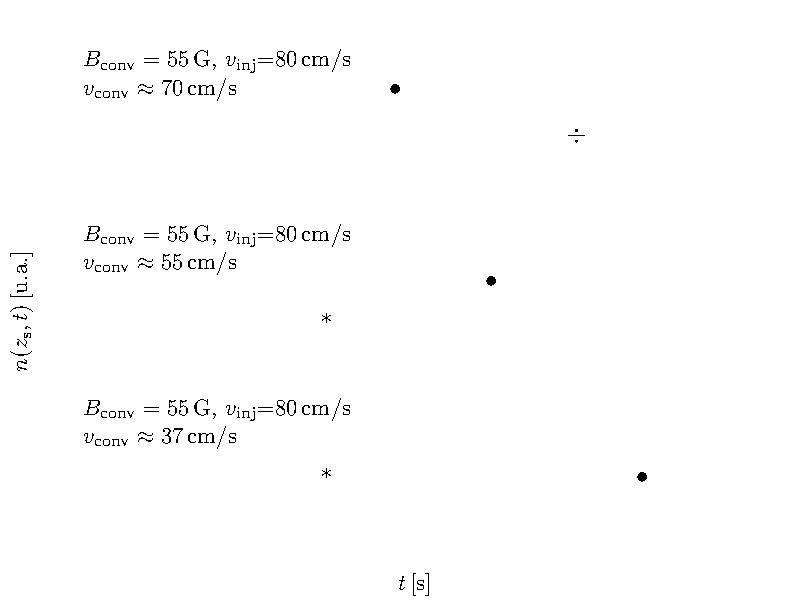
\includegraphics{P2/ConvSignalQP1pktRalenti}
\CaptionFigs{Dans les mêmes conditions que pour la figure~\nref{fig:ConvSignalQP1pkt}, avec $\ConvBamplit=\gauss{55}$, mais pour différentes vitesses du \conv $\vconv < \vinj$. Les pics de détection (repérés par le symbole $\bullet$), localisés autour d'un temps correspondant approximativement à $t=\ttfrac{\zsonde}{\vconv}$ mettent en évidence le piégeage d'atomes dans le \tpqp à la vitesse $\vconv$. On constate cependant que certains atomes ne sont pas piégés et traversent le \tp rapidement (pics repérés par le symbole $\ast$), et d'autres le traversent lentement (pics repérés par le symbole $\div$). Ces phénomènes sont décrits dans la suite (\autoref{sec:InfluenceVitesseConv})}
\label{fig:ConvSignalQP1pktRalenti}
\efigh

\subsubsection{Interprétation des résultats préliminaires}
\noindent Proposons-nous d'interpréter les mesures présentées sur les figures~\nref{fig:ConvSignalQP1pkt} et~\nref{fig:ConvSignalQP1pktRalenti}. Plusieurs points doivent en effet attirer notre attention :
\begin{ditemize}
	\item en l'absence du \tpqp et du fait de l'étalement du \pat lors de sa propagation libre dans le guide, le signal de détection dure plusieurs secondes (figure~\nref{fig:ConvSignalQP1pkt}). En revanche, en présence du \tp on observe un pic de détection localisé autour de $t=\ttfrac{\zsonde}{\vconv}$, qui traduit le fait que l'étalement du paquet a momentanément été \sotosay{gelé}.
	\item pour une faible profondeur des pièges (\gauss{9} sur la figure~\nref{fig:ConvSignalQP1pkt}), une grande partie du signal de détection (correspondant aux atomes les plus lents) reste très proche de celui obtenu sans le \tp. Seule une petite partie des atomes a donc effectivement été piégée%
	\footnote{Ce point est discuté dans la \autoref{sec:InfluenceVitesseConv}.}. 
	\item pour une profondeur plus élevée (\gauss{55} sur la figure~\nref{fig:ConvSignalQP1pkt}), il est possible de piéger presque intégralement les atomes. Nous avons par ailleurs mis en évidence que, si la profondeur est trop élevée, une grande partie des atomes est réfléchie à l'entrée du \tp. Ceux-ci n'atteignent donc jamais le \lsonde et ne sont pas mesurés. Nous avons défini, pour notre \setup, une plage convenable de profondeur des pièges de \gauss{35} à \gauss{55} (voir la \autoref{sec:ConvSimuNum}). 
	\item on constate sur la figure~\nref{fig:ConvSignalQP1pktRalenti} qu'il est possible de ralentir efficacement le \pat. En effet, le temps $t$ d'arrivée du pic de détection correspond au temps attendu si l'on considère que le \p est capturé après \cm{25} de propagation libre. 
	\item si le train va très lentement par rapport à la vitesse d'injection ($\vconv=\cmps{37}$ sur la figure~\nref{fig:ConvSignalQP1pktRalenti}), un deuxième pic de détection apparait (pic repéré par le symbole $*$) et rend compte du fait qu'une partie des atomes est beaucoup trop rapide pour être ralentie par le \tp. 
\end{ditemize}



\section{Obtention d'un \tpIP}\label{sec:ConvTrainIP}

\subsection{Dispositif}
Nous avons mentionné dans la \autoref{sec:ConvTrainAimants} que si le \tpqp permet de transporter des \pats, il est difficilement envisageable de les y refroidir de manière poussée. %De plus le décalage des pièges hors de l'axe du guide  
Cette section montre comment nous pouvons produire un \tp de type \IP, qui se prête particulièrement bien à la manipulation et au refroidissement d'ensembles atomiques ultra-froids.

La solution consiste à superposer au champ du guide et du train d'aimants, un troisième \chm suivant l'axe $z$ du guide. Pour ce faire, nous avons bobiné un solénoïde autour du guide. La figure~\nref{fig:ConvMontageIP} décrit le dispositif. 
\bfigh
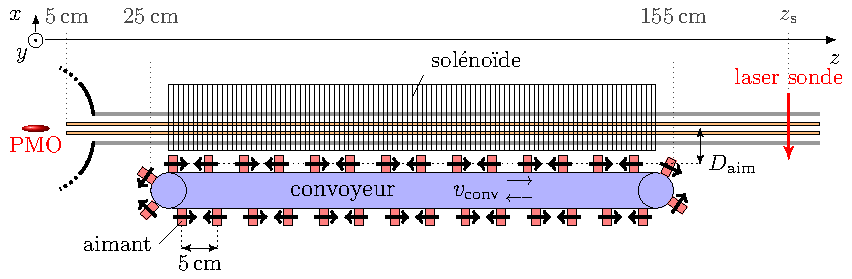
\includegraphics{P2/ConvMontageIP}
\CaptionFigs{Représentation du dispositif permettant de produire un \tpIP. Le solénoïde bobiné autour du guide mesure \m{1} de long et est constitué d'un enroulement de \val{250} spires carrées de $\ConvDSpire = \cm{15}$ de côté (les paramètres intervenant dans le choix de la taille $\ConvDSpire$ des spires sont discutés dans la \autoref{sec:ChoixDimensionSpire}). 
Le \gm n'est pas positionné sur l'axe du solénoïde, mais contre l'une de ses faces intérieures. Ceci est simplement destiné à pouvoir approcher le \conv aussi près que possible de l'axe du guide. L'allure du champ produit sur l'axe du guide est représenté sur la figure~\nref{fig:ConvAnimIPChampLong}.}
\label{fig:ConvMontageIP}
\efigh

La composante longitudinale $\Bpara(z)$ du \chm alors produit sur l'axe du guide est la somme des contributions dues aux aimants et au solénoïde:%
\nome{\ConvBparaSol}{Composante longitudinale du champ produit par le solénoïde}%
\begin{equation}
	\Bpara(z) = \ConvBparaAim(z) + \ConvBparaSol(z)
\virguleformule
	\label{eq:BparaConv}
\end{equation}
%
où il convient de souligner le fait que $\ConvBparaSol(z)$ est toujours du même signe alors que $\ConvBparaAim(z)$ change fréquemment de signe (voir la figure~\nref{fig:ConvAnimQPChampLong}).

\casse

La dépendance en $z$ du champ longitudinal produit par le solénoïde sur l'axe du guide dépend de ses dimensions et de son positionnement par rapport au guide (ce point est discuté dans la \autoref{sec:ChoixDimensionSpire}). En jouant sur ces paramètres et sur le courant traversant le solénoïde, nous pouvons obtenir un champ longitudinal $\Bpara(z)$ dont le signe ne change jamais sur l'axe $z$, tout en présentant des minima locaux (voir la figure~\nref{fig:ConvAnimIPChampLong}). Nous produisons ainsi un \tpIP.
\bfighs
\subfloat{%
\ifthenelse{\NoAnimationsInFigures > 0}{%
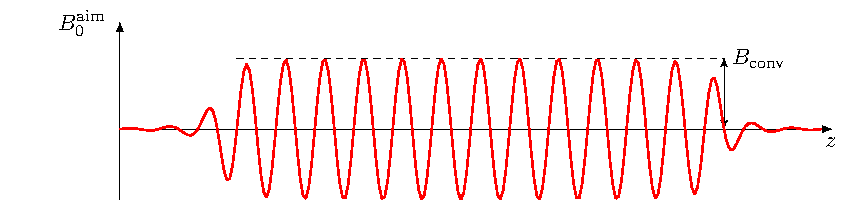
\includegraphics{P2/ConvAnimQPChampLong_1}%
}{%
\animategraphics{10}{images/P2/ConvAnimQPChampLong}{}{}}%
}\\
\RemonteUnPeuFig
\subfloat{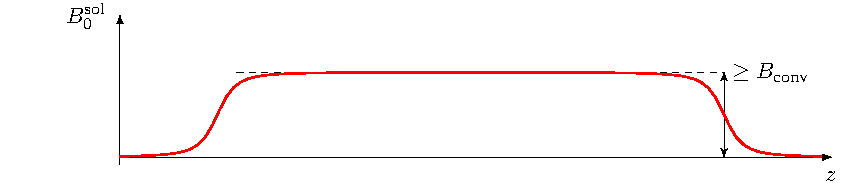
\includegraphics{P2/ConvAnimIPChampLongSol}}\\
\RemonteUnPeuFig
\subfloat{%
\ifthenelse{\NoAnimationsInFigures > 0}{%
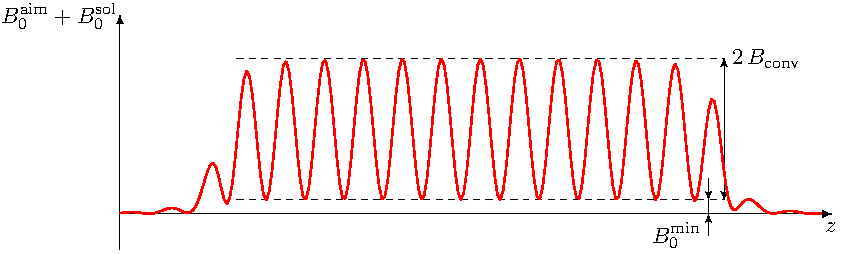
\includegraphics{P2/ConvAnimIPChampLong_1}%
}{%
\animategraphics{10}{images/P2/ConvAnimIPChampLong}{}{}}%
}\\
\CaptionFigss{\AnimateOnline Allure de la composante longitudinale $\Bpara(z)$ du \chm sur l'axe $z$ du guide pour la configuration représentée sur la figure~\nref{fig:ConvMontageIP}.
Ce champ est composé de la contribution $\ConvBparaAim$ des aimants et de celle $\ConvBparaSol$ du solénoïde de manière à produire un \tpIP. Dans cette configuration, le \chm ne s'annule en aucun point. L'espacement entre deux pièges successifs est $\ConvDip = \cm{10}$.}
\label{fig:ConvAnimIPChampLong}
\efigh

\noindent Le module du \chm au fond des puits de potentiel magnétique n'est pas nul, mais vaut:%
\nome{\ConvBparaMin}{Module du \chm au fond des pièges de \IP}%
\begin{equation}
\ConvBparaMin \equiv \ConvBparaSol - \ConvBamplit > 0
\pointformule
	\label{eq:BparaConvMin}
\end{equation}
Le courant parcourant le solénoïde permet d'ajuster précisément la valeur de $\ConvBparaMin$. 
\Resultat{%
En pratique, nous ajustons toujours le courant du solénoïde de manière à avoir $\ConvBparaMin \approx \gauss{1}$, valeur assurant de faible pertes par retournement de spin tout en maintenant un bon confinement transverse des atomes (voir la \autoref{sec:ConfigMagnetiqueGuide}, \vpageref{AN:ValeurB0}).%
}

\casse

\noindent
La configuration de \chm ainsi obtenue fait l'objet de la figure~\nref{fig:ConvChampIP} qui représente, dans le plan horizontal $(x,z)$, quelques lignes de champ ainsi que quelques lignes équipotentielles. 

\Remarque{
Le nombre de \pIPs produit par cette configuration est d'environs $10$, soit deux fois moins que le nombre de \pqps dont il sont issus (voir la \autoref{sec:ConvTrainAimants}). En effet, dans cette configuration, les minima de module du \chm se trouvent face aux aimants dont le champ s'oppose au champ du solénoïde au niveau de l'axe $z$ du guide (ce qui correspond à un aimant sur deux). L'espacement entre deux piège successifs est donc $\ConvDip = \cm{10}$.
}
%
\bfighs
\subfloat{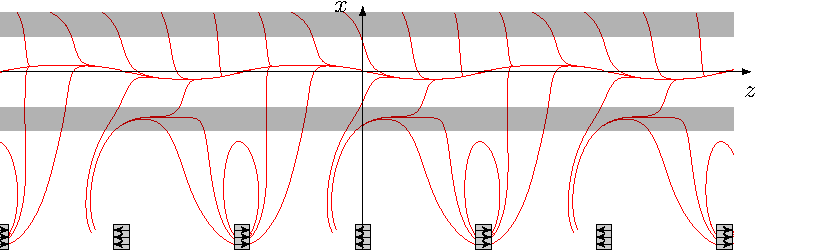
\includegraphics{P2/ConveyerChampMagnetiqueIP}}\\
\subfloat{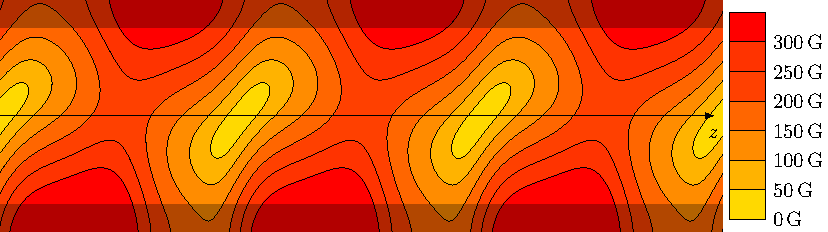
\includegraphics{P2/ConveyerEquipotIP}}
\CaptionFigss{sReprésentation de l'allure de quelques lignes de \chm ainsi que de quelques lignes équipotentielles (suivant lesquelles le module du \chm est constant) pour la configuration décrite sur la figure~\nref{fig:ConvMontageIP}. En superposant le champ produit par les aimants à celui du solénoïde et du \gm nous obtenons une succession de \pIPs sur l'axe du guide. }
\label{fig:ConvChampIP}
\efigh

\casse

\Remarque{
La figure~\nref{fig:ConvChampIP} met en évidence le fait que les \pIPs ne sont pas répartis spatialement de part et d'autre de l'axe $z$ du guide (contrairement aux \pqps). En effet, les extrema de \chm sont maintenant situés, non plus dans des plans médians entre deux aimants successifs, mais dans des plans \emph{passant} par les aimants, là où le champ magnétique transverse $\ConvBtrans$ est très faible%
\footnotemark. 
En conséquence, les \pIPs sont positionnés \emph{sur l'axe $z$ du \gm}, ce qui présente l'avantage de produire des pièges qui passent au centre des \pdecs (voir le chapitre~\nref{chap:Ceramique}).
}
\footnotetext{Le champ magnétique transverse $\ConvBtrans$ est même théoriquement nul dans les plans \emph{passant} par les aimants, si l'on considère une chaîne infinie d'aimants.}


%\casse

\RetireLigne
\subsection{Caractéristiques des \pIPs}

\subsubsection{Profondeur}
Du fait de l'encombrement spatial dû à la présence du solénoïde, la distance $\ConvDaimant$ séparant les aimants de l'axe $z$ du guide est d'au moins \mm{45}.
Pour une configuration avec \val{2} aimants par site et avec $\ConvDaimant=\mm{45}$, l'amplitude des variations de la composante longitudinale du \chm est $\ConvBamplit \approx \gauss{25}$. 

On observe sur la figure~\nref{fig:ConvAnimIPChampLong} que, si le nombre de pièges est divisé par deux, leur profondeur, elle, est doublée. En effet, celle-ci est donnée par l'amplitude \termetech{crête-à-crête} $2\, \ConvBamplit$ des variations de la composante longitudinale du \chm. En utilisant deux aimants sur chaque \scc,  nous pouvons donc obtenir des profondeurs de piège correspondant typiquement à $2\,\ConvBamplit \approx \gauss{50}$.

\nnRemarqueTitre{Fluctuations de la profondeur}{
En plaçant une sonde de \chm aux abords du \conv, nous avons constaté que, d'un piège à l'autre, la profondeur varie typiquement de $5\%$. Ceci est probablement dû à la dispersion des aimantations des aimants. 
Soulignons cependant le fait que ces fluctuations ne sont a priori pas problématiques puisqu'elles concernent une statistique sur l'ensemble des pièges.

En repérant chaque piège lors de son passage devant la sonde, nous avons mesuré,  au fil des passages successifs, des fluctuations typiquement inférieures à $1\%$ pour chaque piège. Ces fluctuations sont à mettre sur le compte des vibrations de la \couconv.
}

\subsubsection{Fréquences d'oscillation}
L'autre caractéristique importante des \pIPs est la force du confinement. C'est la valeur de la composante longitudinale $\ConvBparaMin$ du champ sur l'axe du guide qui détermine la forme du confinement hyperbolique dans le plan transverse%
\footnote{On néglige l'influence du \gtchm produit par les aimants au niveau de l'axe $z$ du guide. Celui-ci est en effet de l'ordre de \gausspcm{20} à comparer à celui fourni par le guide, qui est de typiquement \gausspcm{1000}.}%
. Quant au confinement suivant l'axe longitudinal $z$, il est principalement caractérisé par la profondeur des pièges et leur espacement.

\casse

\ApplicationNumerique{
On peut exprimer le confinement en termes de fréquences d'oscillation des atomes dans le piège. On considère une configuration à deux aimants par site, positionnés à $\ConvDaimant=\mm{35}$ de l'axe $z$, et avec $\ConvBparaMin\approx\gauss{1}$. 
On obtient alors typiquement:
\begin{itemize}
	\item des fréquences d'oscillation selon les axes du plan transverse d'environ \SI{700}{\hertz}, 
	\item et une fréquence d'oscillation suivant l'axe longitudinal d'environ \SI{3}{\hertz}.
\end{itemize}
La moyenne géométrique de ces fréquences d'oscillation, d'environ \SI{120}{\hertz}, est comparable à celle obtenue dans un piège magnétique typique utilisé pour les expériences de \condbe.
}

\subsection{Choix des dimensions du solénoïde}\label{sec:ChoixDimensionSpire}
La mise en place d'un solénoïde permet de maintenir une valeur minimale du \chm au sein du \tp afin de s'affranchir des pertes par retournement de spin. Mais, si le contrôle du courant électrique traversant le solénoïde permet d'ajuster la valeur $\ConvBparaSol$ du \chm produit sur l'axe $z$ du guide, nous allons montrer que ses dimensions ne peuvent pas être choisies arbitrairement. Ce sont elles qui détermineront le taux d'accroissement du champ $\ConvBparaSol$ à l'entrée et à la sortie du solénoïde.

\Remarque{\inlinefig{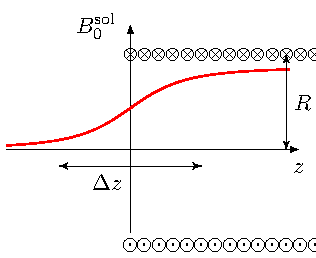
\includegraphics{P2/ConvSolenoideEntreeChamp}}
Le taux d'accroissement du champ magnétique sur l'axe d'un solénoïde dont la longueur est grande devant son rayon répond à une loi du type :
\[
	\ConvBparaSol(z) \propto \frac{z}{\sqrt{z^2+R^2}}+1
	\virguleformule
%	\label{eq:SolenoidChampAxe}
\]
où $R$ est le rayon du solénoïde(voir l'illustration ci-contre). Le champ $\ConvBparaSol(z)$ passe de $10\%$ à $90\%$ de sa valeur maximale sur une distance $\Delta z = \tfrac{8\,R}{3}$.
\picskip{0}
}

%\casse

\noindent Soulignons les points importants qu'il faut garder à l'esprit pour le choix des dimensions du solénoïde:
\begin{itemizel}
	\item nous l'avons dit, le champ \emph{ne doit pas s'annuler} dans le \tpm. Ceci est tout particulièrement vrai \emph{en sortie du train} dans la mesure où, si nous refroidissons les \pats piégés, ceux-ci seront d'autant plus sensibles aux pertes par retournement de spin.
	\item la valeur minimale $\ConvBparaMin$ du \chm au fond des pièges doit rester assez faible, soit environ \gauss{1} afin de \emph{maintenir un bon confinement} transverse. 
	\item en sortie du \tp, les \pats ne doivent \emph{pas être accélérés} par un fort gradient de \chm suivant l'axe longitudinal.
\end{itemizel}

\casse

\noindent
La figure~\nref{fig:ConvAnimIPChampLongDefauts} illustre trois cas caractéristiques d'un mauvais choix des dimensions du solénoïde:
\begin{itemizel}
	\item s'il est de trop faible diamètre, ou trop court, le champ $\ConvBparaSol$ aux extrémités du \tp devient plus faible que l'amplitude $\ConvBparaAim$ des barrières produites par les aimants. On revient alors localement à une configuration de \pqp.
	\item on peut alors être tenté d'augmenter le courant parcourant le solénoïde afin de compenser cet effet aux extrémités du \tp. On a alors une forte valeur de $\ConvBparaMin$ sur toute la longueur du \conv et les atomes sont libérés du \tp dans un fort gradient longitudinal. Ceux-ci subissent donc une forte accélération dans le guide.
	\item enfin, si le solénoïde est de trop grand diamètre, ou trop long, le champ $\ConvBparaSol$ aux extrémités du \tp devient significativement plus élevé que l'amplitude $\ConvBparaAim$ des barrières produites par les aimants. $\ConvBparaMin$ augmente en sortie de \conv et les atomes sont là aussi libérés du \tp dans un fort gradient longitudinal de champ magnétique. 
\end{itemizel}
%
\bfigh
\RemonteUnPeuFig
\subfloat{%
\ifthenelse{\NoAnimationsInFigures > 0}{%
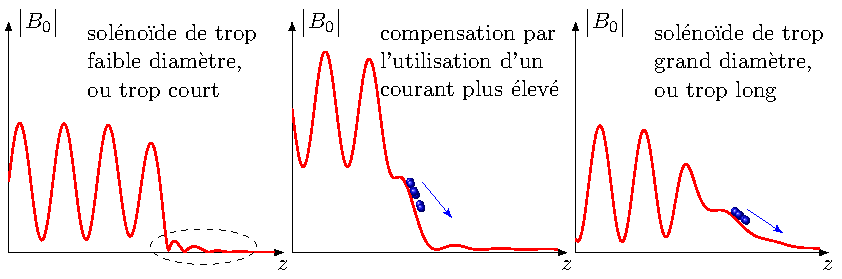
\includegraphics{P2/ConvAnimIPChampLongModuleDefauts_1}%
}{%
\animategraphics{10}{images/P2/ConvAnimIPChampLongModuleDefauts}{}{}}%
}
\CaptionFigss{\AnimateOnline Illustration de trois cas caractéristiques d'un mauvais choix des dimensions du solénoïde. Dans le cas d'un solénoïde trop court ou de diamètre trop faible, le \chm s'annule en sortie du train. Si on compense cet effet en augmentant le courant, le \pat est soumis à une forte accélération longitudinale due à la décroissance brusque du champ. Dans le cas d'un solénoïde trop long ou de diamètre trop élevé, le \pat est libéré du \tp dans un gradient longitudinal de \chm. Il subit là aussi une forte accélération.}
\label{fig:ConvAnimIPChampLongDefauts}
\efigh

Nous avons choisi un diamètre de $\ConvDSpire = \cm{15}$ de manière à voir une montée du champ $\ConvBparaSol$ le long de l'axe $z$ sur une distance $\Delta z \approx \cm{20}$, légèrement supérieure à la distance typique ($\approx \cm{15}$) d'établissement des \bapots dues aux aimants du \conv. 

\vspace{5cm}

\casse


\section{Piégeage d'un \pat dans le \tpIP}\label{sec:Piegeage1pkt}
\Cahier{from : 7,190}
Nous allons maintenant nous intéresser aux piégeage et au refroidissement de \pats dans le \tpIP en mouvement. Notre but est, rappelons le, de capturer les paquets, de manière à momentanément :
\begin{itemize}
	\item limiter la dilution longitudinale afin de maintenir un \tcolel élevé,
	\item recréer des conditions de piégeage tridimensionnel, 
\end{itemize} 
et cela afin de bénéficier d'une évaporation plus efficace. De plus, nous pouvons envisager de ralentir les paquets lors de leur capture de manière à disposer par la suite d'un \jat lent sur la dernière partie du guide.

Lorsque les \pats atteignent le \tpIP en mouvement, ils sont soumis à un potentiel dépendant du temps : des \bapots magnétique s'élèvent sur leur chemin.
%Le but étant de capturer les atomes entre deux de ces barrières, 
Dans cette section, nous nous proposons d'étudier l'influence des différents paramètres intervenant lors de la capture d'un seul \pat par le \tpIP. Afin de souligner les effets physiques mis en jeu lors de ce processus, les observations expérimentales seront mises en rapport avec des résultats de simulations numériques.
Rappelons que les \pats dont il est question dans la suite contiennent typiquement $\val{E9}$ atomes et sont préparés puis injectés dans le guide suivant la procédure décrite dans la \autoref{sec:PaquetsPmo}. 

Trois critères intuitifs peuvent d'ores et déjà être soulignés en ce qui concerne l'alimentation optimale du \tp : 
\begin{itemize}
	\item l'extension longitudinale du paquet doit être sensiblement plus petite que la distance entre deux pièges consécutifs,
	\item le lancement des paquets doit être synchronisé avec le déplacement des pièges, 
	\item la vitesse d'injection du paquet doit être voisine de la vitesse de déplacement du \tpIP.
\end{itemize}
Chacun de ces points fait l'objet d'une sous-section ci-dessous.


\subsection{Extension longitudinale du \pat}
\inlinefig{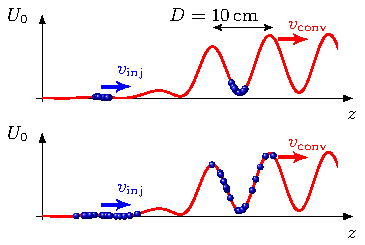
\includegraphics[width=7.cm]{P2/ConvIPExtensionLongi}}
%\RemonteUnPeuFig

\ifthenelse{\FormatEUE > 0}{}
{\AjouteLigne}

Nous considérons dans cette sous-section que la vitesse d'injection $\vinj$ du \p correspond à la vitesse $\vconv$ du \tp.
Si nous voulons avoir \sotosay{une chance} de capturer intégralement un \pat dans l'un des pièges en mouvement, il semble nécessaire que son extension longitudinale soit inférieure à la distance entre deux pièges consécutifs. Sur l'illustration ci-contre nous représentons de manière schématique deux situations. Dans la première, le nuage possède une extension longitudinale suffisamment faible pour être capturé dans l'un des puits de potentiel. Dans la seconde situation il est impossible d'y parvenir et l'on communique, lors du piégeage, une énergie potentielle considérable au \pat.
%\picskip{0}

\casse

Dès l'injection dans le \gm, le \pat commence à s'étaler spatialement du fait de sa \dispvitlong. Comme nous l'avons vu dans le chapitre~\nref{chap:MiroirMobile}, la \templong d'un paquet, une fois injecté dans le guide, est typiquement de $T=\microK{150}$. Ceci correspond à une \dispvitlong :
\begin{equation}
	\deltavjet = \sqrt{\frac{\kb\,T}{m}} \approx \cmps{12}
	\pointformule
	\label{eq:ConvDeltaV}
\end{equation}
\ApplicationNumerique{
La vitesse d'injection $\vinj$ étant voisine de \mps{1}, la distance entre le \pmo et le \tp étant de \cm{25}, le paquet s'étale librement pendant environ \seconde{0,25}. La taille d'un paquet au moment d'atteindre le \tp est donc typiquement de \cm{6}. 
Cette extension longitudinale n'est pas beaucoup plus faible que la distance  $\ConvDip=\cm{10}$ séparant deux pièges consécutifs. Nous montrerons dans la suite (figure~\nref{fig:ConvIP1pktPhase}) que la capture dans ces conditions reste toutefois convenable.
%Une manière d'améliorer ce point serait de rapprocher le plus possible le \conv de la zone du \pmo.
}


\Remarque{
Il convient de noter que notre technique de capture dans un \tpIP a été mise en \oe uvre sur un \setup qui n'avait pas été prévu pour cette tâche lors de sa conception. Les contraintes d'encombrement spatial autour de la chambre du \pmo nous empêchent d'approcher le \conv plus près de l'entrée du \gm.
Le but de nos études consiste précisément en la compréhension des paramètres cruciaux de ce type de méthode, de manière à pouvoir concevoir dans le futur un nouveau dispositif optimisé pour tirer parti au mieux de cette technique.
}
%\Remarque{
%Notre \setup n'ayant initialement pas été prévu pour cette tâche spécifique, et pour des raisons d'encombrement, le \conv ne peut pas être positionné à moins de $z\approx\cm{25}$ du \pmo. 
%%Les \pats ne sont donc \emph{recapturés} dans le \tpqp qu'aprés \cm{25} de propagation libre.
%Un \p injecté dans le guide se propage donc librement dans le guide sur une distance d'environ $\cm{25}$ avant d'être \emph{recapturé} dans le \tpqp. 
%}

 

\subsection{Influence de la synchronisation}\label{sec:ConvInfluenceSynchro}
\inlinefig{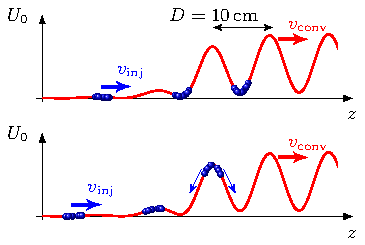
\includegraphics[width=7.cm]{P2/ConvIPCaptureSynchroPetit}}
\RemonteUnPeuFig
Si la taille d'un \pat doit être plus petite que l'espacement entre deux pièges consécutifs, cela ne saurait être une condition suffisante afin de mener à bien la capture dans le \tp. Le \p doit bien entendu arriver au niveau du \conv \sotosay{au bon moment}. Nous représentons ci-contre deux situations faisant intervenir un \pat de faible extension longitudinale. La première représente un \p atteignant le \tp de manière à être entouré de deux \bapots. Dans la seconde situation, le \p arrive une demi-période plus tard et \sotosay{chevauche} une barrière.

\noindent Cette situation est préjudiciable à deux égards:
\begin{itemize}
	\item les atomes du \p vont se séparer de chaque côté de la \bapot,
	\item l'énergie fournie aux atomes lors de l'apparition de la barrière de  potentiel est très élevée.
\end{itemize}

\casse

\subsubsection{Mesures expérimentales}\label{sec:PiegeageMesure1pkt}
Afin de démontrer expérimentalement l'influence de la synchronisation sur le piégeage d'un \pat dans le \tpIP, nous avons mesuré la \datlin $n(\zsonde,t)$ en $\zsonde\approx\cm{100}$, \cad dans la zone couverte par le \conv. 
%Le \lsonde est positionné en $\zsonde\approx\cm{100}$. 
\noindent La figure~\nref{fig:ConvIP1pktPhase} illustre le résultat de deux mesures effectuées en utilisant un \tp dont la profondeur correspond à $2\,\ConvBamplit=\gauss{32}$ et se déplaçant à une vitesse $\vconv=\vinj=\cmps{88}$:
\begin{itemize}
	\item l'une correspondant à un \pat intégralement piégé dans l'un des \pIPs,
	\item l'autre, obtenue avec la même \seqexp, mais en retardant l'injection du \p de \ms{57}. Ce déphasage correspond à la moitié du temps séparant l'arrivée de deux barrières successives.
\end{itemize}
Dans le deuxième cas, les atomes sont clairement séparés en deux ensembles, dans deux pièges contigus. 
Il convient donc de toujours tenir compte de la synchronisation de l'injection des \pats afin d'assurer une capture optimale dans le \tpIP.
%
\bfighss
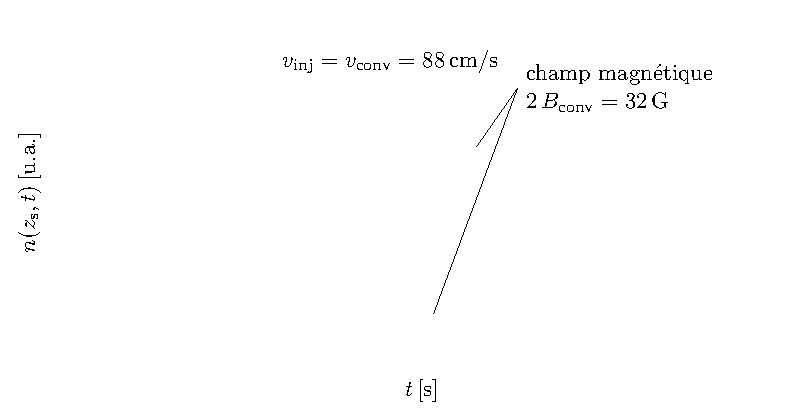
\includegraphics{P2/ConvIP1pktPhase}
\CaptionFigsss{Mesures expérimentales de la \datlin $n(\zsonde,t)$ au sein du \tpIP ($\zsonde\approx\cm{100}$). Le graphe supérieur correspond à une bonne synchronisation de l'injection du \pat, lequel est intégralement capturé dans l'un des \pIPs (la courbe grisée représente le \chm $\Bpara(t)$ au niveau du \lsonde). Sur le graphe inférieur, l'injection est synchronisé de manière à retarder la capture de la moitié du temps séparant deux pièges successifs. Le \pat est alors scindé en deux parties, dans deux pièges contigus. 
}
\label{fig:ConvIP1pktPhase}
\efigh


\casse


\subsection{Influence de la vitesse d'injection}\label{sec:InfluenceVitesseConv}

Jusqu'à présent, nous avons discuté des paramètres influant sur la capture d'un \p dans le \tpIP dont la vitesse $\vconv$ de déplacement est égale à la vitesse d'injection $\vinj$ du \p. Dans cette sous-section, nous abordons le cas d'une capture avec un \conv ayant une vitesse $\vconv\neq\vinj$.

La figure~\nref{fig:ConvIP1pktVitesse} présente des données prises dans des conditions telles que $2\,\ConvBamplit=\gauss{55}$, $\ConvBparaMin=\gauss{1}$, et pour différentes vitesses du \conv : $\vconv = \cmps{115}$, $\cmps{90}$, $\cmps{82}$, $\cmps{65}$, $\cmps{50}$, $\cmps{33}$. Le \lsonde permettant de mesurer la \datlin est positionné \cm{20} en aval du \conv : $\zsonde=\cm{175}$. 
Les temps d'arrivée des pics de détection (repérés par le symbole $\bullet$) ainsi que leur extension temporelle mettent en évidence le piégeage d'une partie substantielle des atomes, et ce sur une \emph{large plage de vitesse}. 
\bfighss
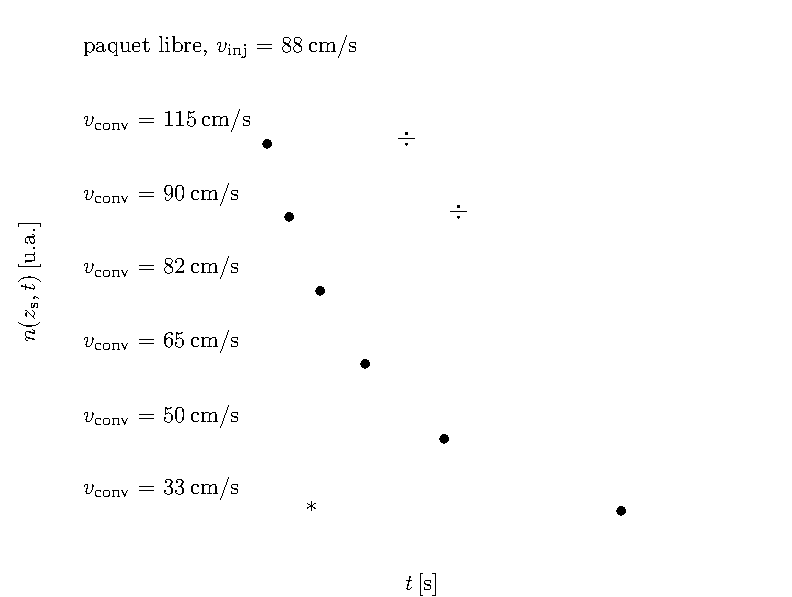
\includegraphics{P2/ConvIP1pktVitesse}
\CaptionFigss{Mesure en fonction du temps suivant l'injection d'un paquet de la \datlin $n(\zsonde,t)$ en aval du \conv ($\zsonde=\cm{175}$). Pour une gamme de vitesses allant de \cmps{33} à \cmps{115} une partie substantielle des atomes est piégée dans le \tpIP (pics de détection repérés par le symbole $\bullet$). Si la vitesse $\vconv$ du \conv est très faible par rapport à la vitesse d'injection $\vinj$ une partie des atomes traverse le \tp presque sans être ralentie (pic de détection repéré par le symbole $\ast$). On constate aussi que certains atomes allant plus lentement que le \conv peuvent traverser le \tp (signaux repérés par le symbole $\div$).}
\label{fig:ConvIP1pktVitesse}
\efigh

\casse

\noindent Soulignons aussi le fait qu'une partie des atomes n'est pas piégée 
%mais traverse le \tpIP presque sans modification de vitesse:
:
\begin{ditemize}
	\item les atomes dont la vitesse est largement supérieure à $\vconv$  ne peuvent être ralentis suffisamment à l'entrée du \tp. Le temps d'arrivée de ces atomes au niveau du \lsonde correspond approximativement au temps d'arrivée d'un \pat libre (signaux repérés par le symbole~$\ast$ sur la figure~\nref{fig:ConvIP1pktVitesse}).
	\vspace{0.5ex}
	\item \inlinefig{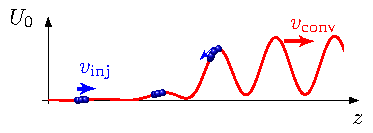
\includegraphics[width=6.cm]{P2/ConvIPAtomesLents}}%
%	\vspace{-.3cm}
	\vspace{0.8ex}
	certains atomes, dont la vitesse est largement plus faible que $\vconv$, peuvent aussi traverser le \tp (signaux repérés par le symbole~$\div$). Bien qu'ayant initialement une faible énergie cinétique, ils peuvent acquérir l'énergie nécessaire lors de l'apparition des \bapots magnétique.%
\picskip{0}
%	\RemonteUnPeuFig
	\item enfin, certains atomes sont réfléchis dès l'entrée du \tp et ne parviennent donc pas jusqu'au \lsonde. La mise en évidence de ces atomes se fait en estimant le nombre d'atomes participant au signal d'absorption, et en le comparant au cas d'un \pat se propageant librement dans le guide (voir la remarque \vpageref[ci-dessous]{Rq:NbrAtomSonde}).
\end{ditemize}

\RemarqueTitre{Estimation du nombre d'atomes piégés}{\label{Rq:NbrAtomSonde}
Le \lsonde permet de mesurer la \datlin en un point du \gm. Pour obtenir le nombre d'atomes concernés par la mesure, il faut effectuer une intégration temporelle du \fat $\flux(\zsonde,t)$. Celui-ci peut être estimé%
\footnotemark%
 :
\begin{itemize}
	\item dans le cas d'un \pat se propageant librement dans le guide par l'expression $\flux(\zsonde,t) = n(\zsonde,t) \, \ttfrac{\zsonde}{t}$. Celle-ci se traduit par le fait que les atomes atteignant le \lsonde en un temps $t$ sont animés d'une vitesse $v = \ttfrac{\zsonde}{t}$.
	\item dans le cas d'atomes piégés dans le \tp et du fait de la faible extension temporelle du signal mesuré, on peut estimer la vitesse des atomes comme étant en moyenne égale à la vitesse du \conv, $\flux(\zsonde,t) = n(\zsonde,t) \, \vconv$.
\end{itemize}
}
\footnotetext{Rappelons que $\zsonde$ est la distance séparant la sonde du \pmo sur l'axe $z$ de propagation des \pats. L'origine des temps correspond au moment de l'injection dans le \gm.}%
\inlinefig{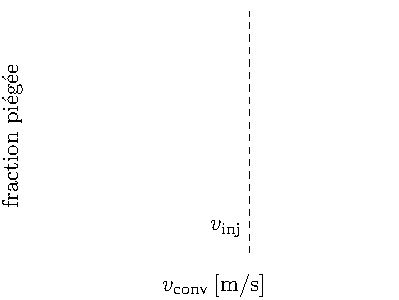
\includegraphics{P2/ConvIP1pktVitesseNumat}}
Pour chaque courbe représentée sur la figure~\nref{fig:ConvIP1pktVitesse}, et en tenant compte de la vitesse des atomes passant devant le \lsonde, nous pouvons estimer la fraction d'atomes piégés dans le \tpIP en fonction de la vitesse $\vconv$ du \conv. Sur le graphe ci-contre, la ligne en trait pointillé représente (en unité arbitraire) une distribution de vitesse gaussienne centrée en $\vinj$ et de variance $\Delta v=\cmps{12}$ (valeur typique pour nos \pats). Celle-ci met en évidence le fait que le \tp fait plus que \sotosay{sélectionner} la fraction d'atomes ayant une vitesse initiale voisine de celle du \conv, \cad que des processus de ralentissement permettent de capturer des atomes ayant une vitesse significativement plus élevée.
%On constate donc qu'une fraction substantiel des atomes peut être piégés dans le \tpIP. %\picskip{0}

\casse

\subsection{Simulations numériques}\label{sec:ConvSimuNum}
Cette sous-section présente le résultats de simulations numériques développées par Antoine Couvert et \dgo, afin de mieux comprendre la physique mise en jeu lors de la capture d'un \pat dans le \tpIP. 

Nous utilisons pour cela une modélisation par un problème unidimensionnel, suivant l'axe $z$, de particules soumises au potentiel $\ConvUaxe(z,t)$ représenté sur la figure \vref{fig:ConvAnimIPChampLong}. L'algorithme de calcul (méthode de Runge-Kunta d'ordre 4) ne fait pas intervenir les collisions entre atomes.
Les conditions initiales des simulations sont choisies de manière à reproduire une distribution $\Distribini(z,\vz)$ gaussienne en position, centrée en $z=0$ (position du \pmo), et en vitesse, centrée sur la vitesse d'injection $\vinj$. La distribution initiale $\Distribini(z,\vz)$ ne fait pas intervenir de corrélation position-vitesse:
% et est caractérisée par seu
\begin{equation}
	\Distribini(z,\vz) = C
	\, \Expo{-\dfrac{z^2}{2\,\Dzini^2}}
	\, \Expo{-\dfrac{\left(\vz-\vinj\right)^2}{2\,\deltavjet^2}}
	\virguleformule
	\label{eq:distribSimu}
\end{equation}
où $C$ est une constante de normalisation.

\inlinefig{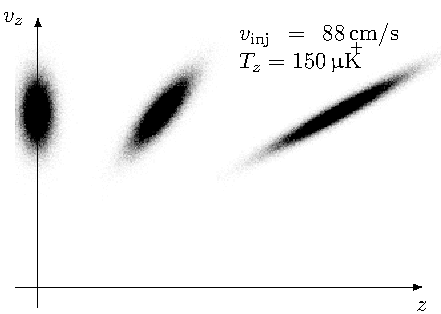
\includegraphics{P2/ConvSimuVi88Initial}}
\noindent Les résultats des simulations numériques seront présentés sous la formes de graphiques dans l'\edpup. Chacun des $\val{E5}$ atomes de la simulation y est repéré par un point ($z,\vz$). 

\noindent L'illustration ci-contre représente la propagation libre d'un \pat à différents instants ($t=0$, $t=\seconde{0.3}$ et $t=\seconde{0.8}$). Pour toutes nos simulations, les conditions initiales sont caractérisées par : 
\begin{itemize}
	\item la vitesse d'injection, $\vinj=\cmps{88}$, 
	\item la \dispvitlong, \\$\deltavjet=\cmps{12}$ (soit $\microK{150}$), 
	\item l'extension longitudinale du \p, $\Dzini=\cm{2}$.
\end{itemize}


\subsubsection{Capture d'un \pat }
Considérons le cas d'un \pat capturé par le \tpIP allant à une vitesse $\vconv=\vinj=\cmps{88}$. La figure~\nref{fig:ConvSimuViVc88_50G} représente l'évolution du \p un temps $t\approx\seconde{1,2}$ après son injection. On y distingue bien les atomes piégés qui évoluent suivant des trajectoires ressemblant à des ellipses dans l'\edpup%
%
\footnote{C'est dans un piège harmonique que les trajectoires dans l'\edp sont rigoureusement elliptiques.}%
.
La synchronisation de l'injection est faite de manière à placer le plus possible d'atomes dans un seul piège (ici, $82\%$ des atomes). 
%
\bfighs
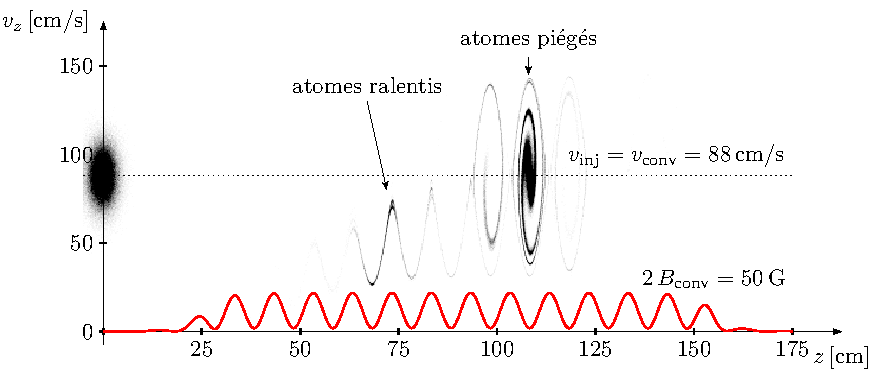
\includegraphics{P2/ConvSimuViVc88_50G}
\CaptionFigs{Représentation de la distribution d'atomes dans l'\edpup à un instant $t \approx \seconde{1,2}$ suivant l'injection du \p dans le \gm. 
La vitesse du \conv est égale à la vitesse d'injection, $\vconv = \vinj = \cmps{88}$.
Le potentiel de piégeage du train au temps $t$ est représenté (en rouge) en unités arbitraires de manière à situer la position des pièges.}
\label{fig:ConvSimuViVc88_50G}
\efigh

La simulation permet de montrer que dans nos conditions expérimentales ($\deltavjet=\cmps{12}$, $\Dzini=\cm{2}$), et même avec une bonne synchronisation, une partie des atomes n'est pas piégée, mais progresse dans le \tp avec une vitesse moyenne inférieure à $\vconv$. 

\casse

\subsubsection{Ralentir un \pat dans le \tpIP}
Nous nous intéressons maintenant au cas du ralentissement d'un \pat lors de la capture dans le \tp. 
La figure~\nref{fig:ConvSimuVi88Vc50} représente les résultats de simulations en prenant une vitesse du \conv $\vconv=\cmps{50}$ inférieure à la vitesse d'injection $\vinj=\cmps{88}$. Trois valeurs différentes de profondeur des pièges sont utilisées. Elle correspondent à des modulations du \chm longitudinale de, respectivement, $2\,\ConvBamplit = \gauss{50}$, $\gauss{20}$ et $\gauss{80}$.
%
\bfigs
\subfloat%[]
{\label{ConvSimuVi88Vc50_a}
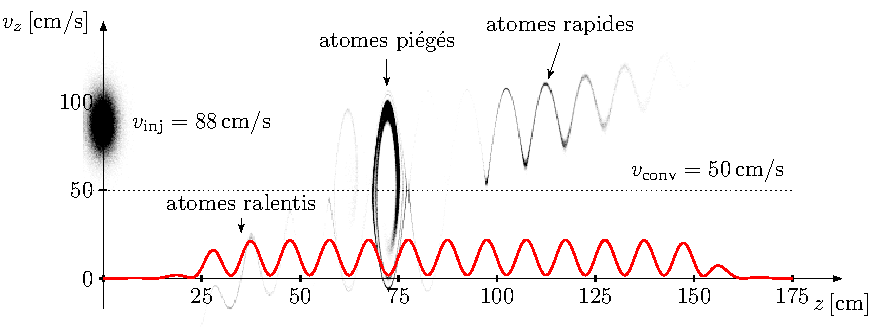
\includegraphics{P2/ConvSimuVi88Vc50_50G}
}\\
\RemonteUnPeuFig
\subfloat%[]
{\label{ConvSimuVi88Vc50_b}
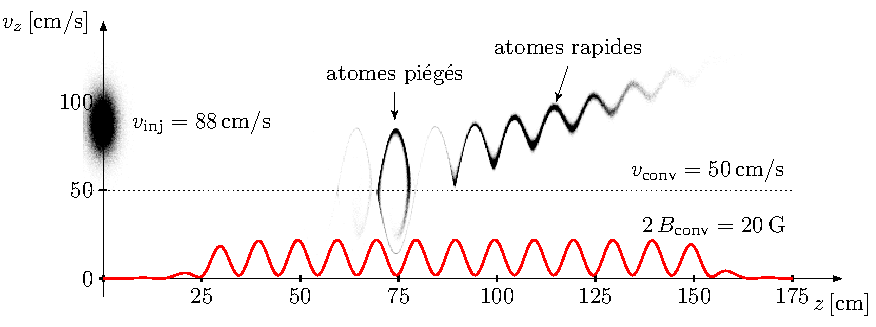
\includegraphics{P2/ConvSimuVi88Vc50_20G}
}\\
\RemonteUnPeuFig
\subfloat%[]
{\label{ConvSimuVi88Vc50_c}
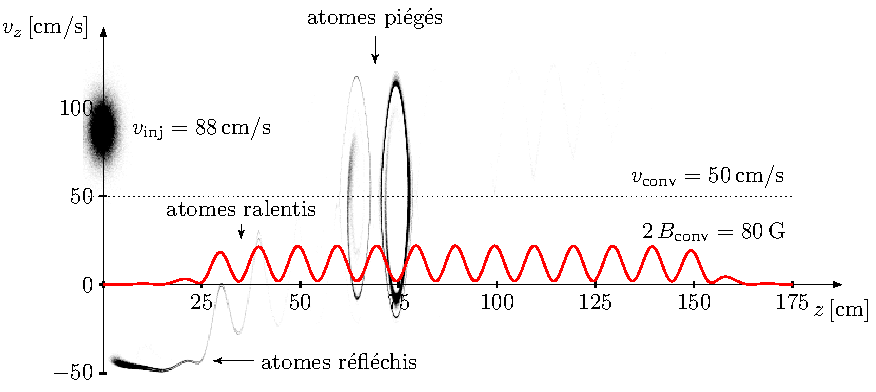
\includegraphics{P2/ConvSimuVi88Vc50_80G}
}
\CaptionFigs{Représentation dans l'\edpup de l'évolution, après un temps $t\approx\seconde{1,2}$,  d'un \pat capturé par le \tpIP. Le \conv est animé d'une vitesse $\vconv=\cmps{50}$, inférieure à la vitesse d'injection du \p, $\vinj=\cmps{88}$. Chaque graphique correspond à une valeur différente de la profondeur des pièges (correspondant à $2\,\ConvBamplit = \gauss{50}$, $\gauss{20}$ et $\gauss{80}$). Le potentiel de piégeage du train au temps $t$ est représenté (en rouge) en unités arbitraires de manière à situer la position des pièges.}
%\label{fig:ConvSimuVi88Vc50_50G}
\label{fig:ConvSimuVi88Vc50}
\efig
%
On peut ainsi distinguer les trois comportements typiques mis en évidence expérimentalement sur la figure \vref{fig:ConvIP1pktVitesse}:
\begin{ditemize}
	\item pour une hauteur de barrière trop faible (\gauss{20}), une fraction importante des atomes, les plus \emph{rapides}, ne peuvent être suffisamment ralentis par les \bapots à l'entrée du \tp. Ces atomes traversent alors chaque piège du train avec une vitesse moyenne supérieure à $\vconv$.
%
\ApplicationNumerique{Évaluons la vitesse relative $\vrel\equiv v -\vconv$ d'un atome de \Rb abordant le \tp afin que celui-ci passe avec certitude au dessus des \bapots. Pour $2\,\ConvBamplit=\gauss{20}$, on a :
	\begin{equation}
	\frac{1}{2}\,m\,\vrel^2 = 2\,\ConvBamplit\,\mu 
	\mbox{~,~ soit $\vrel \approx \cmps{35}$}
	\pointformule
	\label{eq:VrelConv20G}
\end{equation}
Or, dans la simulation numérique de la figure~\nref{fig:ConvSimuVi88Vc50}, environ $60\%$ des atomes possèdent une vitesse initiale supérieure de $\cmps{35}$ à celle du \conv%
\footnotemark%
. On comprend donc bien pourquoi la majorité d'entre eux passent au dessus de toutes les barrières.%
}
\footnotetext{Si le fait d'avoir une vitesse relative supérieure à $\vrel$ est une condition \emph{suffisante} pour traverser tous les pièges, ce n'est pas une condition \emph{nécessaire}. En effet, certains atomes possédant une vitesse initiale trop faible peuvent acquérir beaucoup d'énergie s'ils \sotosay{chevauchent} une barrière lors de son apparition à l'entrée du train. Ce phénomène est directement lié à la taille et la synchronisation du \pat à l'entrée du \tp (voir la \autoref{sec:ConvInfluenceSynchro}).}
%
	\item lorsqu'on augmente la hauteur des \bapots, cette catégorie d'atomes rapides et non-piégés disparait progressivement. 
	\ApplicationNumerique{Le même calcul que précédemment avec $2\,\ConvBamplit=\gauss{50}$ donne $\vrel \approx \cmps{45}$ : seulement $5\%$ des atomes possèdent une vitesse initiale suffisante pour assurer une traversée des barrières.}%
	En contrepartie, certains atomes subissent un tel ralentissement à l'entrée du \tp que leur vitesse moyenne devient très faible. Ces atomes, dans le référentiel en mouvement lié au \conv se propagent en sens inverse, et traversent aussi les barrières.
%
	\item si on augmente trop la hauteur des barrières (\eg \gauss{80}), on constate qu'il est même possible de réfléchir une fraction importante des atomes à l'entrée du \tp. Ce résultat est intéressant dans la mesure où il est difficile de mesurer expérimentalement le nombre d'atomes réfléchis puisque ceux-ci n'atteignent jamais le \lsonde. Le mécanisme physique mis en jeu est bien entendu du type de celui que nous avons décrit dans le chapitre~\nref{chap:MiroirMobile} traitant de la réflexion d'un \pat sur un \mimamo.
\end{ditemize}

\Resultat{
L'analyse numérique qui fait l'objet des figures~\nref{fig:ConvSimuViVc88_50G} et~\nref{fig:ConvSimuVi88Vc50} permet de distinguer trois types de trajectoires atomiques dans l'\edpup: 
\begin{itemize}
	\item les atomes qui possèdent initialement ou qui acquièrent suffisamment d'énergie pour passer au dessus des \bapots du \tp, 	
	\item les atomes qui sont ralentis lors de l'entrée dans le \tp si bien que leur vitesse moyenne est inférieure à celle du \conv. Ces atomes passent aussi au dessus des \bapots en se propageant plus lentement que le \tp. Si la hauteur des barrières est grande, on peut même réfléchir une partie des atomes.
	\item enfin, les atomes capturés dans l'un des pièges.
\end{itemize}
}





\section{Piégeage et refroidissement de \patss}
Nous avons montré que notre technique permet de capturer et de transporter efficacement un \pat dans un \tpIP.  Dans cette section nous exposons les résultats relatifs au piégeage de plusieurs \ps simultanément, ainsi que de leur \rpef. C'est en effet cet aspect que nous cherchons à mettre en valeur dans le contexte de notre expérience de production et d'évaporation d'un \jatuf.

\casse

\subsection{Injection répétée de \pats}
Pour démontrer l'efficacité du piégeage de \pats injectés successivement, nous plaçons le \lsonde en $\zsonde\approx\cm{100}$ afin de mesurer la \datlin $n(\zsonde,t)$ dans le \tp (comme dans la \autoref{sec:PiegeageMesure1pkt} où il s'agissait du piégeage d'un \p).
La figure~\nref{fig:ConvIPMultiPakets} illustre deux mesures expérimentales effectuées dans le cas d'une injection périodique, \val{4,4} fois par seconde:
\begin{itemize}
	\item la première est effectuée en l'absence du \conv. On y observe comme prévu%
	\footnote{Voir le chapitre~\nref{chap:JetAtomique}.}
	la formation d'un \jat continu, résultat du recouvrement des \pats qui se propagent librement dans le guide.
	\item la seconde est effectuée en présence du \tpIP%
	\footnote{Dans les \seqexps en question, l'injection de chaque \p est synchronisée avec le \conv de manière à optimiser le chargement des pièges.}
	ayant une profondeur donnée par $2\,\ConvBamplit=\gauss{32}$ et animé d'une vitesse $\vconv=\vinj=\cmps{88}$.
\end{itemize}
%
\bfighs
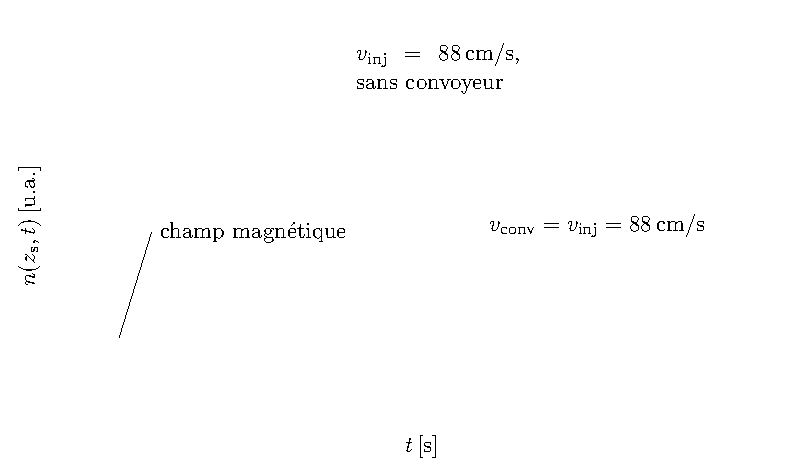
\includegraphics{P2/ConvIPMultiPakets}
\CaptionFigs{Mesure de la \datlin $n(\zsonde,t)$ au sein du \tpIP ($\zsonde\approx\cm{100}$). Le graphe supérieur correspond, en l'absence du \conv, à la formation d'un \jat continu obtenu par le recouvrement de \pats injectés \val{4,4} fois par seconde (voir la \autoref{sec:FormationJetContinu}). Le graphe inférieur correspond lui aux mêmes conditions expérimentales, mais en présence du \tpIP animé d'une vitesse $\vconv=\vinj=\cmps{88}$, le tout étant convenablement synchronisé (voir la \autoref{sec:PiegeageMesure1pkt}). L'échelle verticale est identique pour les deux graphes. Le fait qu'un piège sur deux soit vide prouve que chaque \pat est capturé intégralement dans un piège donné. La \datlin est plus élevée dans les pièges (d'un facteur 2 à 3) que dans le \jat obtenu dans les mêmes conditions.
}
\label{fig:ConvIPMultiPakets}
\efigh

\Resultat{%
Nous observons donc non-seulement le piégeage individuel de chaque \p dans le \tpIP, mais aussi et surtout, que la \dat est plus élevée dans les pièges (d'un facteur 2 à 3) que dans le \jat en absence de \conv. Ce dernier point, synonyme d'un \tcoli élevé, est très important dans la perspective de mettre en \oe uvre le \rpef des \ps durant leur transport. Le \tcolel moyen par atome dans les pièges est estimé à environ $\SI{10}{\reciprocal\second}$.
}

\subsection{Échauffement dû à la capture dans le \tp}\label{sec:EchauffCaptureConv}
Avant de présenter les résultats relatifs au refroidissement de \pats piégés dans le \tpIP, nous soulevons dans cette sous-section un point essentiel relatif à la capture des \ps.  
En effet, ceux-ci subissent alors une compression, et il en résulte une augmentation de leur température. Cet effet est d'autant plus marqué que les \ps possèdent une grande extension longitudinale.
Réciproquement, à la sortie du convoyeur, une décompression longitudinale et un refroidissement prennent place. 


\subsubsection{Échauffement lors d'une capture instantanée des \pats}
Essayons de comprendre les processus physiques à l'origine de l'échauffement. Nous envisageons pour cela le cas d'une capture instantanée des \pats, \cad en considérant que ceux-ci sont soumis à l'apparition brusque des pièges magnétiques. Nous supposerons de plus que la synchronisation de l'injection est parfaite, \cad que le \cdm du \p se place exactement au fond du piège. 
%Dans ces conditions, nous nous proposons d'estimer l'échauffement du \p lors de la capture si sa taille de ce
\Remarque{
Cette situation ne correspond pas précisément à ce qui se produit lors de la capture dans le \tp puisque les \bapots se forment progressivement (en quelques dixièmes de seconde typiquement). Cependant, une telle étude simplifiée permet de se rendre compte des ordres de grandeur des énergies mises en jeu lors de la capture.
} 
\inlinefig{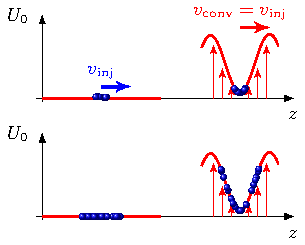
\includegraphics[width=6cm]{P2/ConvIPExtensionLongiChauffage}}
\noindent \begin{minipage}{9.3cm}
\noindent La figure ci-contre illustre le mécanisme de chauffage d'un \pat du fait de son extension longitudinale finie en considérant deux cas :
\begin{itemize}
	\item celui d'une faible extension longitudinale du \p, 
	\item celui d'une extension longitudinale comparable à l'espacement $\ConvDip$ entre pièges. 
\end{itemize}
Au moment ou les barrières apparaissent, les atomes se voient fournir une énergie potentielle d'autant plus élevée que ceux-ci explorent une large plage du dit potentiel. Dans le cas où la taille du \p est comparable à la distance $\ConvDip$ entre deux pièges (soit \cm{10}) on peut estimer le gain d'énergie comme étant de l'ordre de la valeur moyenne du potentiel $\MoyenneBraKet{\ConvUaxe}$. 
\end{minipage}
\vspace{0.1cm}
\picskip{1}

\ApplicationNumerique
{Considérons un \pat dont l'extension longitudinale au moment du piégeage est d'environ \cm{10}. 
%Nous choisirons une distribution gaussienne de variance $\Delta x=\cm{3}$ pour la position des atomes au sein du \p. 
En prenant les conditions exposées ci-dessus, avec des pièges dont la profondeur est donnée par $2\,\ConvBamplit=\gauss{35}$, l'énergie potentielle acquise en moyenne par chaque atome en entrée est de l'ordre de :
\[
	\MoyenneBraKet{\ConvUaxe} 
	= \muB\,\ConvBamplit
%	\frac{
%	\Integrale{\ConvUaxe(x)\,\Expo{\dfrac{-x^2}{2\,\Delta x}}}{\dx}
%	}{
%	\Integrale{\Expo{\dfrac{-x^2}{2\,\Delta x}}}{\dx}
	\approx \SI{5E{-27}}{\joule} \pointformule 
	%\,\,\,\mbox{ce qui correspond à environ \microK{350}} \nonumber
%	\label{eq:ConvUaxeMoyen}
\]
Cette énergie correspond, en terme de température, à $\MoyenneBraKet{\ConvUaxe} = \kb\,\Tlong$ avec \mbox{$\Tlong \approx \microK{350}$}.
}
%
N'oublions pas qu'une fois les atomes capturés, l'énergie potentielle acquise selon l'axe $z$ longitudinal va se redistribuer sur tous les degrés de liberté%
\footnote{
Nous avons en effet vu que le \tcolel moyen par atome dans les pièges est estimé à environ $\SI{10}{\reciprocal\second}$, ce qui autorise une \reth rapide.}%
. 
Afin d'étudier de problème, on devrait donc considérer :
\begin{itemize}
	\item les $3$ degrés de liberté en vitesse,
	\item les $2$ degrés de liberté transverses dans un \pc linéaire,
	\item et le degré de liberté longitudinal selon lequel on modélise le piégeage par un confinement harmonique.
\end{itemize}
Après \reth il ne resterait ainsi plus qu'un quart de l'énergie potentielle acquise selon l'axe longitudinal (se reporter à la remarque sur le théorème du viriel, \vpageref{Rq:Viriel}). 

\subsubsection{Limites de la modélisation unidimensionnelle}
D'après la modélisation simple que nous venons de décrire, nous pourrions conclure que la température du \p augmenterait donc finalement d'au plus \microK{80}. 

\noindent \emph{Cependant}, il convient ici de rappeler que si la \templong $\Tlong$ des \ps est d'environ \microK{150} juste après leur injection, la \tempt, elle, est beaucoup plus élevée (de l'ordre de \microK{600}) du fait de la compression non-adiabatique à l'entrée du \gm (voir la \autoref{sec:EntreeGuideNonAdiabatique}). 
\Resultat{
Quand on considérait des \ps se propageant librement, la \reth était négligée (voir la \autoref{sec:EntreeGuideNonAdiabatique}). Dans le \tp, il faut en tenir compte et conclure que la \templong des \pats augmente bien, mais surtout du fait de la \reth avec les degrés de liberté transverses, sur lesquels beaucoup d'énergie \thiq est disponible. La \templong des \ps atteint une valeur de l'ordre de \microK{500}.
}

%En sortie du \tp, la disparition soudaine des barrières emporte avec elle l'énergie potentielles longitudinale sans conduire à un refroidissement dans la mesure où l'énergie restante est déjà bien répartie sur les autres degrés de liberté.
\EnFaitNon{
Nos simulations montrent qu'un paquet initialement sans dispersion de vitesse longitudinale, mais dont l'extension est comparable à la distance entre deux pièges successifs, ressort du \tp avec une dispersion de vitesse longitudinale de l'ordre%
\footnote{L'amplitude des \bapots magnétique utilisée pour ces simulations correspond à $2\,\ConvBamplit=\gauss{35}$. Ces simulations se base sur une modélisation par un problème à une dimension.}%
 de $\Delta v = \cmps{10}$, ce qui correspond à une température $\Tlong\approx\microK{100}$.
Après \reth, \cad après la redistribution de cette énergie sur les degrés de liberté transverses, cet excès de température est de \microK{20}. 
Un paquet dont la taille initiale est plus petite subit naturellement un moindre échauffement. 
}

\EnFaitNon{
II - 3 - c - Énergie des particules piégées. Sortie du convoyeur.
Les simulations révèlent également un autre effet d'autant plus prononcé que l'énergie des particules piégées est élevée. Il s'agit d'une légère accélération des particules à la sortie du convoyeur. Pour nos paramètres expérimentaux, la température du jet produit en l'absence de convoyeur est de l'ordre de \microK{600}. Nos mesures réalisées après la sortie du convoyeur confirment qu'elle n'est pas affectée par la présence du convoyeur. 
}

\RetireLigne

%\subsubsection{Simulation nu}
\subsubsection{Mesures expérimentales de température}
Nous avons effectué des mesures de \tempt sur le \jat au bout du \gm (voir la \autoref{sec:MesureTempTrans}). Nous estimons ainsi mesurer la température $T$ du jet puisque ce dernier a eu le temps d'évoluer vers l'\eqthdy durant les trois derniers mètres de propagation. Dans des conditions expérimentales typiques%
\footnote{Se reporter à la \autoref{sec:FormationJetContinu} pour le détail des conditions expérimentales typiques.}%
, avec une injection des \pats à une vitesse $\vinj=\mps{1}$, nous comparons deux cas expérimentaux:
\begin{itemize}
	\item en l'absence de \conv, la \tempt du jet mesurée est $T=\microKpm{600}{20}$,
	\item en présence du \tpIP animé d'un mouvement uniforme à une vitesse $\vconv=\vinj=\mps{1}$, et dont la profondeur correspond à $2\,\ConvBamplit=\gauss{35}$, nous mesurons  $T=\microKpm{590}{20}$.
\end{itemize}
%
\Resultat{%
Nous ne détectons donc pas de variations mesurables de température dues au \tp, dans la limite de la précision dont nous disposons pour la mesure de la \tempt du jet.
}

%\RemarqueTitre{Un autre démon de Maxwell}{
%En toute rigueur, il faudrait même s'attendre à mesurer une température du \jat plus faible en présence du \tp. En effet, si l'échauffement à l'entrée du train est relativement faible, la température longitudinale $\Tlong$ y augmente beaucoup du fait de la \reth avec les autres degrés de liberté et atteint $\Tlong=\Teq\approx\microK{500}$. Or, en sortie du train, le refroidissement dû à la décompression se fait en proportion de la température $\Teq$. On reprend donc plus d'énergie à chaque \pat que ce qu'on en a fournie.
%
%ET DONC UNE PHRASE DEMON DE MAXWELL QUI SERA ECRITE APRES AVOIR REPRIS LA FIN DU CHAPITRE MIROIR !
%}

\subsection{Refroidissement par \evap dans le \tp}
Le transport multiple de \pats dans le \tp de type \IP se prête fort bien à la mise en \oe uvre du refroidissement par évaporation. Afin de démontrer ceci expérimentalement nous avons placé quatre antennes \rfs sur le tube de verre du guide magnétique dans la zone couverte par le \conv. La mise en \oe uvre de cette technique est décrite dans la \autoref{sec:EvapRf}. Chaque paquet atomique piégé traverse ainsi successivement quatre zones d'évaporation durant son transport. Nous mesurons l'effet de l'évaporation sur la \tempt $\Ttrans$ du jet ainsi obtenu en bout de \gm.

\Resultat{
L'évaporation des \ps durant leur transport nous a ainsi permis de réduire la température du \jat par un facteur $2$ (passant de \microK{590} à \microK{280}). Le \fat est quant à lui réduit d'un facteur $4$. Nous pouvons ainsi estimer le gain en \ddedpup%
\footnotemark%
:
\begin{equation}
	\frac{\rhojetaxeapres}{\rhojetaxe} \approx \val{2}
	\pointformule
	\label{eq:GainPsdConv}
\end{equation}
\finformule
}
\footnotetext{On se reportera à la \autoref{sec:GuidageJet} pour le calcul du gain en \ddedpup sur l'axe du \jat.}

\section{Conclusion}

Grâce à un agencement périodique d'aimants permanents fixés sur un \conv longeant le guide, nous avons produit un \tpIP mobiles. Les paquets d'atomes injectés dans le guide sont re-capturés longitudinalement puis relâchés \m{1,2} en aval. Ce dispositif permet de contourner les trois difficultés majeures liées à la manipulation d'un \jatuf 
%pour le \rpef 
que nous avons mentionnées à la fin du chapitre~\nref{chap:JetAtomique}. 
Nous avons en effet démontré expérimentalement que la capture dans le \tp en mouvement permet de :
\begin{itemize}
	\item limiter la dilution longitudinale afin de maintenir un \tcolel élevé,
	\item recréer des conditions de piégeage tridimensionnel, 
\end{itemize} 
et cela afin de bénéficier d'une évaporation plus efficace. De plus, nous pouvons envisager de ralentir les paquets lors de leur capture de manière à disposer, par la suite d'un \jat lent sur la dernière partie du guide.

Nous avons de plus mis en \oe uvre le \rpef sur $5$ paquets simultanément et avec une alimentation périodique du \tp. Ceci constitue une première dans notre communauté et ouvre diverses perspectives, comme la parallélisation de la production de \becs. 
Ces expériences nous ont  en outre permis de définir les paramètres critiques qui permettront sans doute la mise au point d'un futur \setup entièrement optimisé pour l'usage de cette technique. 


On peut toutefois se demander si notre technique, qui fait intervenir des pièces mécaniques mobiles soumises à d'inévitables vibrations, resterait exploitable s'il s'agissait de refroidir des \pats jusqu'à des température beaucoup plus faibles. 
En particulier, un \bec résisterait-il aux vibrations du dispositif?
%, notamment de la courroie du \conv?


